\section{Evaluation}
\label{evaluation}

We have conducted experiments to demonstrate the effectiveness of our approach. In this section, we present the experimental results of our analysis on various JavaScript benchmarks.

%We conducted three sets of experiments to demonstrate several aspects of our analysis. (1) the ability for the localization algorithm to pinpoint the critical bottleneck of the analysis on JavaScript libraries, (2) further experiments of the localization algorithm on JavaScript benchmarks and demonstrate the ability of suggestion algorithm, and (3) a case study on using our analysis to localize the issues of an unscalable and imprecise analysis for analyzing jQuery, and demonstrate that with manual modifications of the program without changing the semantics, the same analysis manages to be scalable on analyzing the jQuery programs.
\begin{comment}
\begin{table*}[h!]
\centering
\begin{tabular}{ | C{0.68in} | C{0.4in} | C{0.4in} | C{0.4in} | C{0.4in} | C{0.4in} | C{0.4in} | C{0.4in} | C{0.4in} | C{0.4in} | C{0.4in} | C{0.4in} |}
\hline
 {\bf library} & \multicolumn{3}{|c|}{\bf baseline} &  \multicolumn{4}{|c|}{\bf straw man} &  \multicolumn{4}{|c|}{\bf selective}\\
 \hline
 & {\tt REAC\_} {\tt FUNC} & {\tt AVG\_} {\tt TARG} & {\tt HIGH\_} {\tt POLY} & {\tt REAC\_} {\tt FUNC} & {\tt AVG\_} {\tt TARG} & {\tt HIGH\_} {\tt POLY} & time (sec) & {\tt REAC\_} {\tt FUNC} & {\tt AVG\_} {\tt TARG} & {\tt HIGH\_} {\tt POLY} & time (sec)\\ 
 \hline
jQuery & 291 & 20.1 & 272 & 206 & 1.2 & 21 & 17.3 & 206 & 1.2 & 16 & 16.9\\
 \hline
 prototype.js & 418 & 12.3 & 124 & 170 & 1.3 & 18 & ~2.9 & 170 & 1.3 & 18 & ~3.2\\
 \hline
 yui & 244 & ~9.8 & 124 & 101 & 1.1 & ~2 & ~1.1 & 101 & 1.1 & ~2 & ~2.0 \\
 \hline
 \end{tabular}
\caption{\textmd{Benchmarks I precision and performance results.}}
\vspace{-6pt}
\label{table:b1-precision-time}
\end{table*}
\end{comment}

\begin{table*}[th!]
\centering
\begin{tabular}{ | C{0.80in} | C{0.4in} | C{0.4in} | C{0.4in} | C{0.4in} | C{0.4in} | C{0.4in} | C{0.4in} | C{0.4in} | C{0.4in} | C{0.4in} |}
\hline
 {\bf library} & \multicolumn{3}{|c|}{\bf 1-CFA} &  \multicolumn{3}{|c|}{\bf 1-CFA + 1st-arg-sens} &  \multicolumn{4}{|c|}{\bf 1-CFA + selective 1st-arg-sens}\\
 \hline
 & {\tt REAC\_} {\tt FUNC} & {\tt AVG\_} {\tt TARG} & {\tt HIGH\_} {\tt POLY} & {\tt REAC\_} {\tt FUNC} & {\tt AVG\_} {\tt TARG} & {\tt HIGH\_} {\tt POLY} &  {\tt REAC\_} {\tt FUNC} & {\tt AVG\_} {\tt TARG} & {\tt HIGH\_} {\tt POLY} & time (sec)\\ 
 \hline
jQuery & 312 & ~2.2 & 441 & 206 & 25.0 & 1235 & 206 & 1.2 & 16 & 16.3\\
 \hline
 prototype.js & 451 & 12.9 & 259 & 170 & ~3.3 & ~124 & 170 & 1.5 & 39 & ~2.9\\
 \hline
 script.aculo.us & 617 & 14.4 & 188 & 179 & ~2.7 & ~145 & 179 & 1.4 & 47 & ~4.6 \\
 \hline
 \end{tabular}
\caption{\textmd{Benchmarks I precision and performance results.}}
\vspace{-6pt}
\label{table:b1-precision-time}
\end{table*}

\subsection{Experimental Setup} 

\subsubsection{Metrics}

In our evaluation, we compare the performance and precision of points-to analysis. A JavaScript points-to analysis usually constructs a call graph as well as a points-to graph. For precision on a call graph, we measure (i) {\tt HIGH\_POLY}: the number of highly polymorphic call sites (i.e., call sites with more than 5 targets), (ii) {\tt AVG\_TARG}: the number of targets averaged over all call sites, and (iii) {\tt REAC\_FUNC}: the number of reachable functions. The {\tt HIGH\_POLY} and {\tt REAC\_FUNC} metrics were also used by Sridharan et al. \cite{Sridharan:2012:CTP:2367163.2367191} to evaluate the call graph construction algorithms. For precision on a points-to graph, we measure {\tt PTS\_SIZE}: the overall points-to size (i.e., the total number of points-to set sizes over all local variables in the program; the points-to set of a variable is the number of abstract objects, represented by the allocation sites, it refers to). 
%For each of the above metrics, if an analysis $A_1$ produces smaller results than another analysis $A_2$, $A_1$ is more precise than $A_2$ on that aspect of the call graph or points-to graph.
In addition, we measure the performance of the points-to analysis with its running time (in seconds).

%{\bf Call graph metrics.} no. of high polymorphic call sites, average no. of targets, reachable functions

%{\bf Points-to graph metrics.} overall points-to size

\subsubsection{Benchmarks}

We use two sets of JavaScript benchmarks in our evaluation.
%For the JavaScript benchmarks experiments presented in Section \ref{}, we used the benchmarks collected by Kashyape \cite{}. There are 28 programs in the benchmarks that are divided into 4 categories. As demonstrated by Wei and Ryder \cite{}, programs from different categories can benefit from different context-sensitive analysis; thus in our experiments, we compared the precision and performance of whole-program context-sensitive analyses with the selective context-sensitive analysis to demonstrate the effectiveness of our bottleneck localization.

%For the JavaScript library experiments presented in Section \ref{}, we used the benchmarks developed by Srihadran \cite{}. The libraries that we evaluated are jQuery, prototype.js, and .... Because there is no existing analysis in WALA can scale (given the budget of 10 minutes) to analyze the simple applications that use the original versions of these libraries, we use manually transformed versions of these libraries which scale only with the analysis presented by Srihadran \cite{}. Each of the libraries is associated with several simple applications.

%For the previous two experiments, we have used a specific version of WALA to perform the evaluation. In the current WALA, there exist no analysis that can finish analyzing the programs used in the second experiments. In our case study presented in Section \ref{}, we use our bottleneck localization algorithm to pinpoint the places the these library applications that the current WALA analysis resulted in significant imprecision and manually transform the programs without changing their semantics so that the analysis is more precise on analyzing the transformed programs. A similar approach is used by Srihadran \cite{} to investigate the effectiveness of correlation tracking analysis.

{\bf Benchmarks I.} Benchmarks I consists of applications that use JavaScript libraries, generated by Sridharan et al. \cite{Sridharan:2012:CTP:2367163.2367191}. In this benchmark, there are 11, 5 and 1 simple web applications that invoke {\it jQuery}, {\it prototype.js} and {\it script.aculo.us} libraries, respectively. These libraries are among the most popular JavaScript libraries for developing real-world web applications, especially {\it jQuery} \cite{LibraryUsage}. As reported by Sridharan et al. \cite{Sridharan:2012:CTP:2367163.2367191}, an analysis without the specialized argument sensitivity experienced severe performance and precision problems; it required advanced static analysis techniques as well as manual code rewriting for improving precision and performance. In our experiments, we reuse these libraries with these manual transformations.

{\bf Benchmarks II.} Benchmarks II are JavaScript applications collected by Kashyap et al. \cite{Kashyap:2014:JSA:2635868.2635904}. Twelve out of the 28 programs from the original benchmarks were selected for our evaluation. These programs are collected from open-source JavaScript repositories, standard JavaScript benchmarks (e.g., SunSpider\footnote{https://webkit.org/perf/sunspider/sunspider.html}), and the Emscripten LLVM test suite\footnote{http://kripken.github.io/emscripten-site/}, the results of which benefit from various context-sensitive analyses \cite{Kashyap:2014:JSA:2635868.2635904,DBLP:conf/ecoop/WeiR15}.

\subsubsection{Experimental Design} 
%We have designed experiments to illustrate the effectiveness of the important aspects of our approach.

{\bf Root-cause localization.} We perform experiments on Benchmarks I to illustrate the accuracy of the root-cause localization algorithm. In this experiment, we use WALA's whole-program 1-CFA analysis as the {\it baseline} analysis, which experiences scalability and precision problems for the JavaScript library applications. For each of the Benchmark I programs, we perform the localization algorithm on the 1-CFA analysis, localizing a set of functions that contain the root causes. We then apply additional argument sensitivity on the first arguments (i.e., 1st-argument sensitivity \cite{DBLP:conf/ecoop/WeiR15}) of all these functions; for the rest of the functions, the 1-CFA analysis is performed (i.e., a 1-CFA and {\it selective} 1st-argument-sensitive analysis). We compare the precision results among the 1-CFA, the whole-program 1-CFA and 1st-argument-sensitive analysis, and the {\it selective} analysis using the call graph metrics for Benchmarks I. We also compare the differences in terms of analysis performance.

%In our experiments, we use WALA's whole-program 1-CFA and 0-1-CFA JavaScript points-to analyses\footnote{For the results reported in Sections \ref{b1-res} and \ref{b2-res}, we conducted the experiments based on analyses implemented under WALA version R\_1.3.4. We performed the case studies in Section \ref{case-study} using the up-to-date WALA implementations to locate and understand the root causes.} as the {\it baseline} analyses for Benchmarks I and Benchmarks II, respectively. The 1-CFA analysis experiences scalability and precision problems for the JavaScript library applications in Benchmarks I and the 0-1-CFA analysis is imprecise for the programs in Benchmarks II comparing to other analyses in comparison. A whole-program combined context-sensitive analysis (i.e., 1-CFA and argument sensitivity) applies the more accurate but also more expensive context sensitivity policy. 

%{\bf Root-cause localization.} To illustrate the accuracy of the root-cause localization approach, for each of the benchmark programs, we perform the localization algorithm on the {\it baseline} analysis where performance and/or precision problems are present. We apply 1-CFA analysis and combined 1-CFA and argument-sensitive analysis on all the functions that contain the identified root causes for Benchmarks I and Benchmarks II, respectively; for the rest of the functions, the {\it baseline} analysis is performed (i.e., a {\it selective} context-sensitive analysis). We compare the precision results among the {\it baseline}, whole-program combined context-sensitive analysis, and {\it selective} analyses using the call graph metrics for Benchmarks I and points-to results metrics for Benchmarks II. We also compare the differences in terms of analysis performance.

%In addition, we use a combined context-sensitive analysis (i.e., 1-CFA and argument sensitivity) as the {\it straw man} analysis, which often results in significant precision improvement comparing to the {\it baseline} analysis results for most of the benchmark programs. To illustrate the accuracy of the root cause localization approach, for each of the benchmark programs, we apply the localization algorithm on the {\it baseline} analysis where performance and/or precision problems are present. For all the functions that contain the identified root causes, we apply the same context-sensitive policies as the {\it straw man} analysis; for the rest of the functions, the {\it baseline} analysis is performed (i.e., a {\it selective} combined 1-CFA and argument-sensitive analysis).  We compare the performance and precision results among the {\it baseline}, {\it straw man}, and {\it selective} analyses using the call graph and points-to results metrics.

{\bf Improvement suggestion.} For the programs in Benchmarks II, we apply the root-cause localization as well as improvement suggestion algorithms on the {\it baseline} 0-1-CFA analysis. We execute each program to obtain a program trace. A root cause function may be suggested to apply (i) a context-insensitive analysis, (ii) a single context-sensitive analysis (i.e., 1-CFA or argument sensitivity on any argument of the function\footnote{Object sensitivity \cite{Milanova:2005:POS:1044834.1044835} applies calling contexts on the receiver argument.}), or (iii) a combined context-sensitive analysis (e.g., 1-CFA and 1st-argument sensitivity). Based on the suggestion results, we automatically use the suggested analysis for the root cause functions; for the rest of the functions, the 0-1-CFA analysis is performed (i.e., a {\it auto-selective} context-sensitive analysis). We compare the performance and precision results of the {\it auto-selective} analysis with the 0-1-CFA analysis and the {\it full-sensitive} analysis (i.e., a whole-program combined context-sensitive analysis that applies 1-CFA and argument sensitivity on all arguments) for Benchmarks II to illustrate the effectiveness of the improvement suggestion.

%\footnote{Because the dynamic analysis could not produce traces for {\it aha} and {\it llubenchmark} in Benchmarks II, we have applied 1-CFA and argument sensitivity on all arguments for all the root cause functions in these two programs.}

%For the programs in Benchmarks II, we apply the root-cause localization as well as improvement suggestion algorithms on the {\it baseline} 0-1-CFA analysis. Based on the suggestion results, we automatically use the suggested context-sensitive analysis for the specific functions; for the rest of the functions, the {\it baseline} analysis is performed (i.e., a {\it auto-selective} context-sensitive analysis). We compare the performance and precision results of the {\it auto-selective} analyses with other analyses for Benchmarks II to illustrate the effectiveness of the improvement suggestion.

The experimental results were obtained on a 2.5 GHz Intel Core i5 MacBook Pro with 16 GB memory running the Mac OS X 10.11 operating system.

%{\bf Hypotheses.}
%Hypothesis 1: our bottleneck localization algorithm is capable of pinpointing the specific locations in the analyzed program that resulted in significant imprecision.
%Hypothesis 2: our suggestion algorithm can accurately identify the functions in the programs that need the specific context sensitivity for precision.

\subsection{Benchmarks I Results}
\label{b1-res}

Tables \ref{table:b1-precision-time} and \ref{table:b1-characteristics} show the experimental results of Benchmarks I. For each JavaScript library, the results are arithmetically averaged over all the applications that use the specific library. For example, the 291 reachable functions of {\it jQuery} library from the 1-CFA analysis (i.e., column 2 of the jQuery row in Table \ref{table:b1-precision-time}) is calculated by averaging the number of reachable functions the 1-CFA analysis obtained for all 11 {\it jQuery} applications.\footnote{Because the applications in Benchmarks I are relatively simple programs that use the JavaScript libraries, the analysis performance and precision results of these programs are dominated by the underlying libraries. Therefore, we report the average results based on the corresponding libraries.} 

{\bf Precision and performance.} Table \ref{table:b1-precision-time} shows the precision and performance results of the analyses on Benchmarks I. Columns 2-4, 5-7, and 9-11 show the results of call graph precision metrics for the 1-CFA analysis, the whole-program combined 1-CFA and 1st-argument-sensitive analysis (i.e., {\it whole-combined} analysis), and the 1-CFA and {\it selective} 1st-argument-sensitive analysis, respectively. For each analysis, we present its number of reachable functions (i.e., columns 2, 5, and 8), average number of targets per call site (i.e., columns 3, 6 and 9), and the number of highly polymorphic call sites (i.e., columns 4, 7, and 10). In addition, column 11 show the points-to analysis time in seconds of the {\it selective} analysis. Given the time budget of 10 minutes, both the 1-CFA analysis and the {\it whole-combined} analysis failed to complete analyzing any of the programs in Benchmarks I; therefore, their precision results were calculated from the incomplete call graphs obtained after the timeout.

The {\tt REAC\_FUNC} results of the {\it whole-combined} and the {\it selective} analyses in Table \ref{table:b1-precision-time} are the same for all three libraries, which are significantly more precise than those of the 1-CFA analysis. Only 29\% (for {\it script.aculo.us}) to 66\% (for {\it jQuery}) functions considered reachable by the 1-CFA analysis are produced by the {\it whole-combined} and the {\it selective} analyses. Interestingly, the number of highly polymorphic call sites is below 50 for the {\it selective} analysis for all three libraries, while the 1-CFA analysis produces 188 (for {\it script.aculo.us}) to 441 (for {\it jQuery}) and the {\it whole-combined} analysis results in 145 (for {\it script.aculo.us}) to 1235 (for {\it jQuery}) highly polymorphic call sites. This result suggests that (i) 1-CFA analysis is imprecise to resolve the call targets in many cases, and (ii) because the {\it whole-combined} analysis applies 1st-argument sensitivity over all the program, it may create many calling contexts for the functions that are not identified as roots causes which may not significantly increase the analysis precision (e.g., in terms of the {\tt REAC\_FUNC} metric). The average number of targets per call site from the {\it selective} analysis ranges from 1.2 (for {\it jQuery}) to 1.5 (for {\it prototype.js}), indicating the {\it selective} analysis precisely resolves the targets for most call sites. Although the {\it whole-combined} analysis reduces the {\tt AVG\_TARG} of the 1-CFA analysis from 12.9 to 3.3 and from 14.4 to 2.7 for {\it prototype.js} and {\it script.aculo.us}, respectively, it still results in higher average number of targets per call site comparing to the {\it selective} analysis. For {\it jQuery} library, applying argument sensitivity over all the program results in significant increase of {\tt AVG\_TARG} (i.e., on average 25 targets per call site) and {\tt HIGH\_POLY} (i.e., 1235 highly polymorphic call sites) due to the additional calling contexts.

The last column in Table \ref{table:b1-precision-time} shows that the {\it selective} analysis finishes analyzing the libraries on average between 3 seconds (for {\it prototype.js}) and 16 seconds (for {\it jQuery}). Due to the fact that the 1-CFA analysis could not finish analyzing any of these libraries under 10 minutes, we claim that the {\it selective} analysis has significantly better performance because of the precision gained by applying 1st-argument sensitivity on the root cause functions. The {\it whole-combined} analysis also could not complete within the 10-minute time budget. Applying 1st-argument sensitivity over all the program generates too many calling contexts for the propagation system to converge. In summary, the results in Table \ref{table:b1-precision-time} suggest that (i) our root-cause localization algorithm is capable of locating the functions where the 1-CFA analysis experiences significant precision and performance loss, and (ii) because the root causes are highly condensed in these JavaScript libraries (see more discussions below), applying the 1st-argument-sensitive analysis only on the localized functions achieved a much better balance between precision and performance comparing to the {\it whole-combined} analysis.

% call graph precision results of the {\it straw man} and the {\it selective} analyses in Table \ref{table:b1-precision-time} are the same, except for the number of high polymorphic call sites from {\it jQuery} library. Because the {\it straw man} analysis applies 1-CFA and argument-sensitive analysis over all the program, it may create more calling contexts for the functions that are not identified as root causes than the {\it selective} analysis, resulting in more targets in terms of call graph nodes for some call sites. On the other hand, the {\it selective} analysis is significantly more precise than the {\it baseline} analysis on all three JavaScript libraries. The {\it selective} analysis reduces the number of reachable functions computed by the {\it baseline} analysis by 29\% (for {\it jQuery}) to 59\% (for {\it prototype.js} and {\it yui}). The average number of targets per call site from the {\it selective} analysis ranges from 1.1 (for {\it yui}) to 1.3 (for {\it jQuery}), indicating the {\it selective} analysis precisely resolves the targets for most call sites, while the {\it baseline} analysis reports on average at least 9.8 targets per call site. Comparing to the {\it baseline} analysis, the {\it selective} analysis also results in significantly fewer call sites with more than 5 targets, reducing the number by at least an order of magnitude.

%Column 12 in Table \ref{table:b1-precision-time} shows that the {\it selective} analysis finishes analyzing the libraries on average between 2 seconds (for {\it yui}) and 17 seconds (for {\it jQuery}). Due to the fact that the {\it baseline} analysis could not finish analyzing any of these libraries under 10 minutes, we claim that the {\it selective} analysis has significantly better performance and scalability. Consistent with the precision results, the performance results of the {\it straw man} and the {\it selective} analyses are similar. In summary, the results in Table \ref{table:b1-precision-time} suggest that (i) our root cause localization algorithm is capable of locating the functions where the {\it baseline} analysis experiences significant precision and performance loss, and (ii) because the root causes are highly condensed in these JavaScript libraries (see more discussions below), applying the context-sensitive analysis only on the localized functions achieved very similar results comparing to the {\it straw man} analysis.

\begin{table}[t!]
\centering
\begin{tabular}{ | C{0.8in} | C{0.6in} | C{0.72in} | C{0.6in} |}
\hline
 {\bf library} & {\bf no. of localized functions} & {\bf no. of evaluations} &  {\bf slope} \\
 \hline
jQuery & 2 & 25000 & 3.7 \\
 \hline
 prototype.js & 4 & 72000 & 5.1 \\
 \hline
 script.aculo.us & 4 & 96000 & 4.9 \\
 \hline
 \end{tabular}
\caption{\textmd{Root-cause localization results of Benchmarks I.}}
\vspace{-6pt}
\label{table:b1-characteristics}
\end{table}

{\bf Root-cause localization characteristics.} Table \ref{table:b1-characteristics} shows additional information that characterizes the results of the root-cause localization algorithm. For the experiments on Benchmarks I, we paused the 1-CFA analysis every 1000 evaluations to decide if the root-cause localization algorithm should be performed. Columns 2, 3, and 4 present the number of functions identified as root causes, the number of evaluations until performing root-cause localization, and the slope of the last 1000 evaluations (i.e., the increase in the total number of points-to relations divided by 1000), respectively. 

Our algorithm identifies 2, 4 and 4 functions as root causes for {\it jQuery}, {\it prototype.js}, and {\it script.aculo.us}, respectively. Comparing to the number of reachable functions computed by any analysis in Table \ref{table:b1-precision-time} (i.e., more than 150 functions), very small fractions of these functions were identified as root causes. This result as well as the good precision and performance of the {\it selective} analysis support our intuition that a small number of complex constructs in the programs may contribute to significant loss of analysis performance and precision if not handled accurately. Therefore, it is useful for our automated localization algorithm to pinpoint these root causes, as shown.

Column 4 shows that the slopes of the last 1000 evaluations range from 3.7 (for {\it jQuery}) to 5.1 (for {\it prototype.js}). For example for {\it prototype.js}, the large slope indicates that the precision of the 1-CFA analysis significantly decreases during this period (i.e., about 5 new points-to relations per constraint), while the slope of the simple linear regression for all previous evaluations is 0.9. This result suggests that our heuristics accurately decide when to perform the root-cause localization for JavaScript libraries.

%We report the results via (1) the performance/precision of 01cfa, whole-program 1cfa+parameter and selective 1cfa+parameter, (2) investigation of the localization results (i.e., number of selected functions/all functions, and the number of iteration that starts the evaluation).

%So 1 table (i.e., precision/time results of the analyses) and another table (i.e., localization results).

\begin{figure*}[th!]
        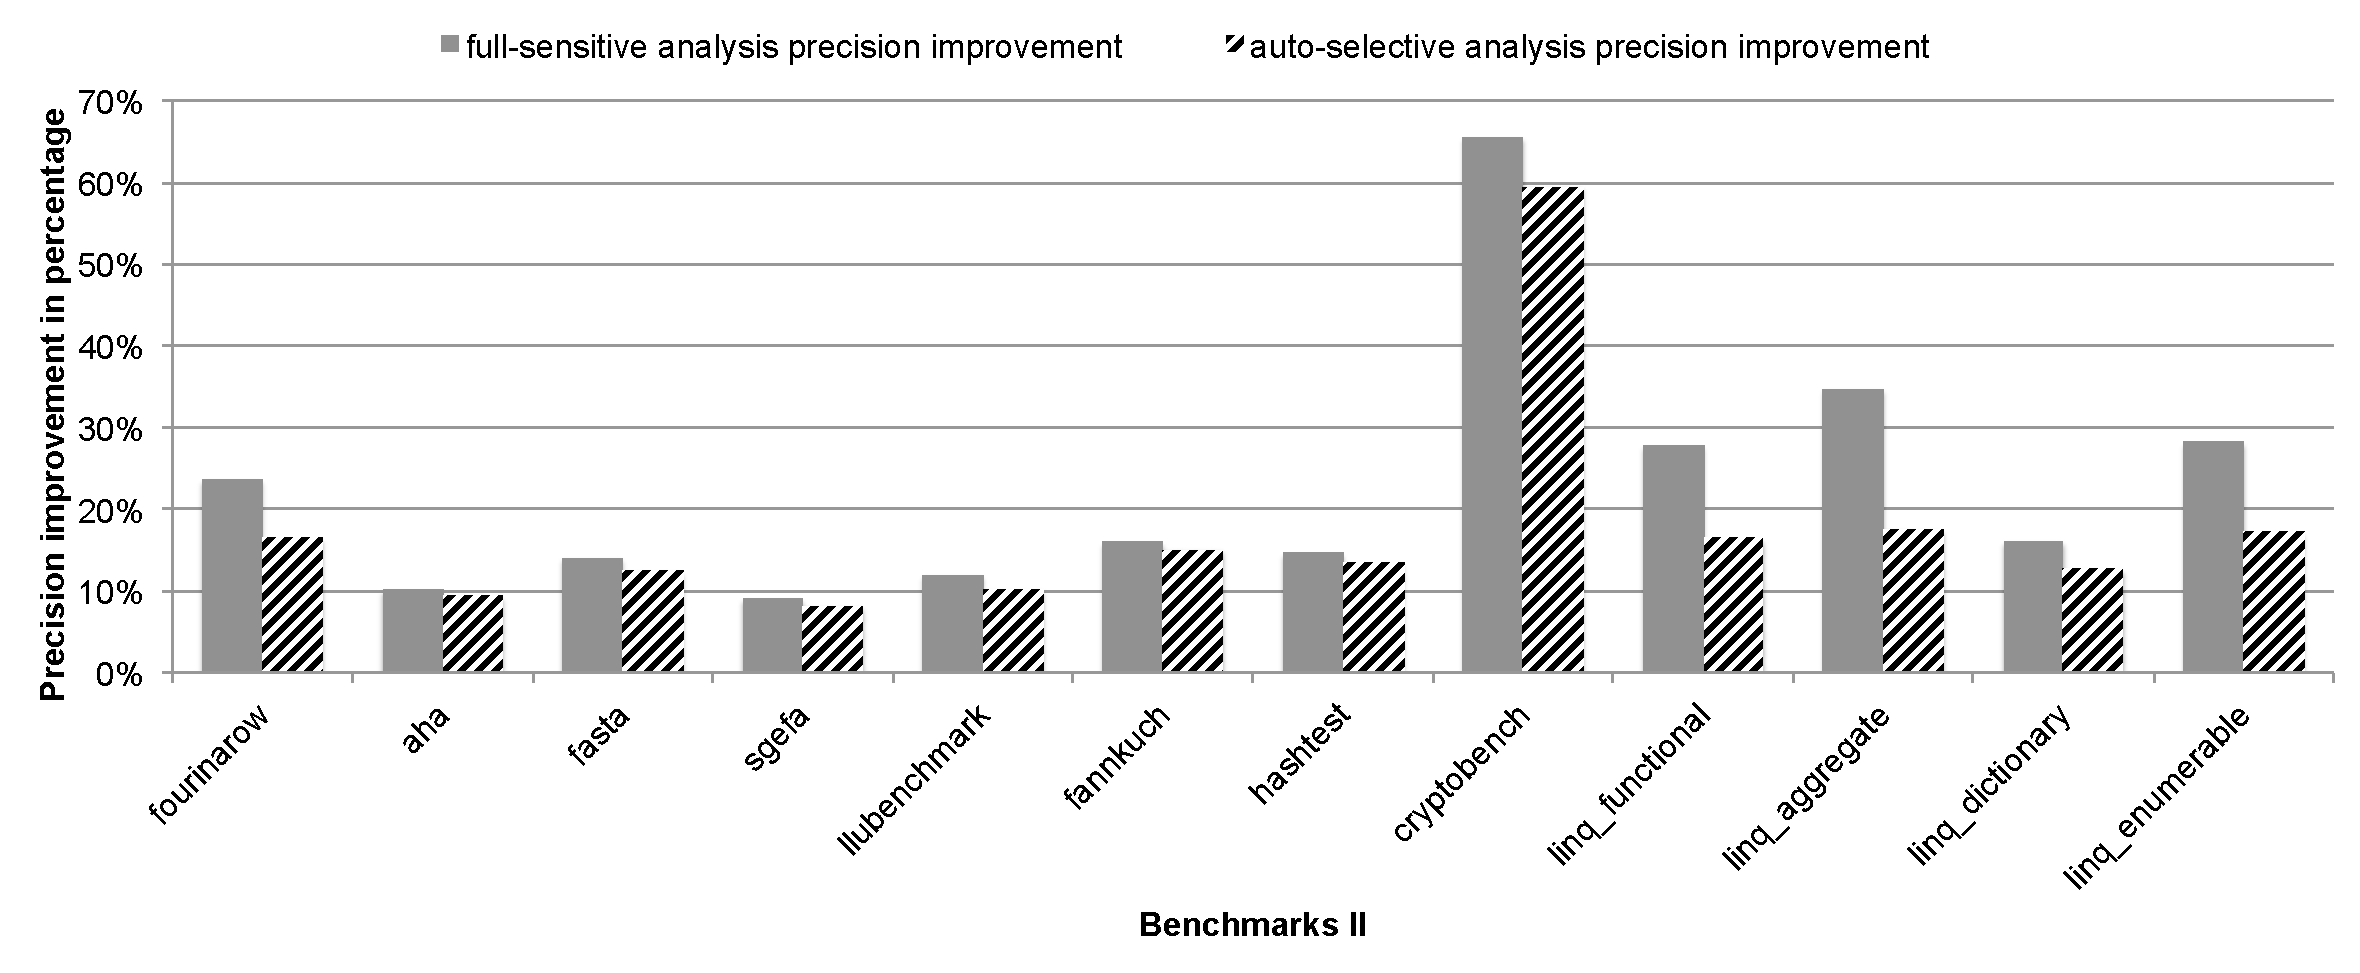
\includegraphics[width=2\columnwidth]{b2-precision}
\caption{\textmd{Benchmarks II precision results.}}
\vspace{-6pt}
\label{fig:b2-precision}
%\vspace{-6pt}
\end{figure*}

\subsection{Benchmarks II Results}
\label{b2-res}

Figures \ref{fig:b2-precision} and \ref{fig:b2-performance} show the precision and performance results of Benchmarks II, respectively. Because the 0-1-CFA analysis finishes analyzing all 12 programs in Benchmarks II within the time budget of 10 minutes, the root-cause localization was performed after the 0-1-CFA points-to analysis completes on each program.

Figure \ref{fig:b2-precision} presents the {\tt PTS\_SIZE} precision improvement of the {\it full-sensitive} analysis (i.e., grey bars) and the {\it auto-selective} analysis (i.e., patterned bars) over the 0-1-CFA analysis. Because the {\it full-sensitive} analysis applies 1-CFA and argument sensitivity of all arguments over all the functions, its results are at least as precise as the {\it selective} analysis. In Figure \ref{fig:b2-precision}, the y axis shows the precision improvement of the corresponding analysis {\tt Y} over the 0-1-CFA analysis {\tt 0-1-CFA}, calculated as follows

\[
  {\tt IMP_{Y} = {{PTS\_SIZE_{0-1-CFA} - PTS\_SIZE_{Y}} \over {PTS\_SIZE_{0-1-CFA}}} \times 100\%}
\]

Therefore, {\tt IMP\textsubscript{Y}} measures analysis {\tt Y}'s precision in terms of removing the false positives from the 0-1-CFA analysis results. In Figure \ref{fig:b2-precision}, the {\it whole-combined} analysis improves the {\tt PTS\_SIZE} precision over the 0-1-CFA analysis by between 9\% (for {\it sgefa}) to 65\% (for {\it cryptobench}). For all but five programs (i.e., {\it fourinarow}, {\it cryptobench}, {\it linq\_functional}, {\it linq\_aggregate} and {\it linq\_enumerable}), the differences of the precision improvement percentages are within 3.5\% between the {\it full-sensitive} and the {\it auto-selective} analyses, indicating that the {\it auto-selective} analysis produces similar results to the {\it full-sensitive} analysis for most programs. The results of the {\it linq\_functional} program exhibit the largest difference in terms of precision improvement (i.e., 17\%) between the {\it full-sensitive} 35\%) and the {\it auto-selective} (18\%) analyses. Nevertheless, more than 50\% of the false positives that are produced by the 0-1-CFA analysis, but not the {\it full-sensitive} analysis, are absent from the {\it auto-selective} analysis results for this program.

Figure \ref{fig:b2-performance} presents the performance results of the {\it full-sensitive} (i.e., grey bars) and the {\it auto-selective} (i.e., patterned bars) analyses comparing to the 0-1-CFA analysis performance. The y axis shows the overhead of the corresponding analysis {\tt Y}'s time cost comparing to the 0-1-CFA analysis time (i.e., ${\tt \frac{TIME_{Y}}{TIME_{0-1-CFA}}}$). The performance of an analysis on each benchmark program was obtained by averaging over 30 repeated executions.

\begin{figure*}[th!]
        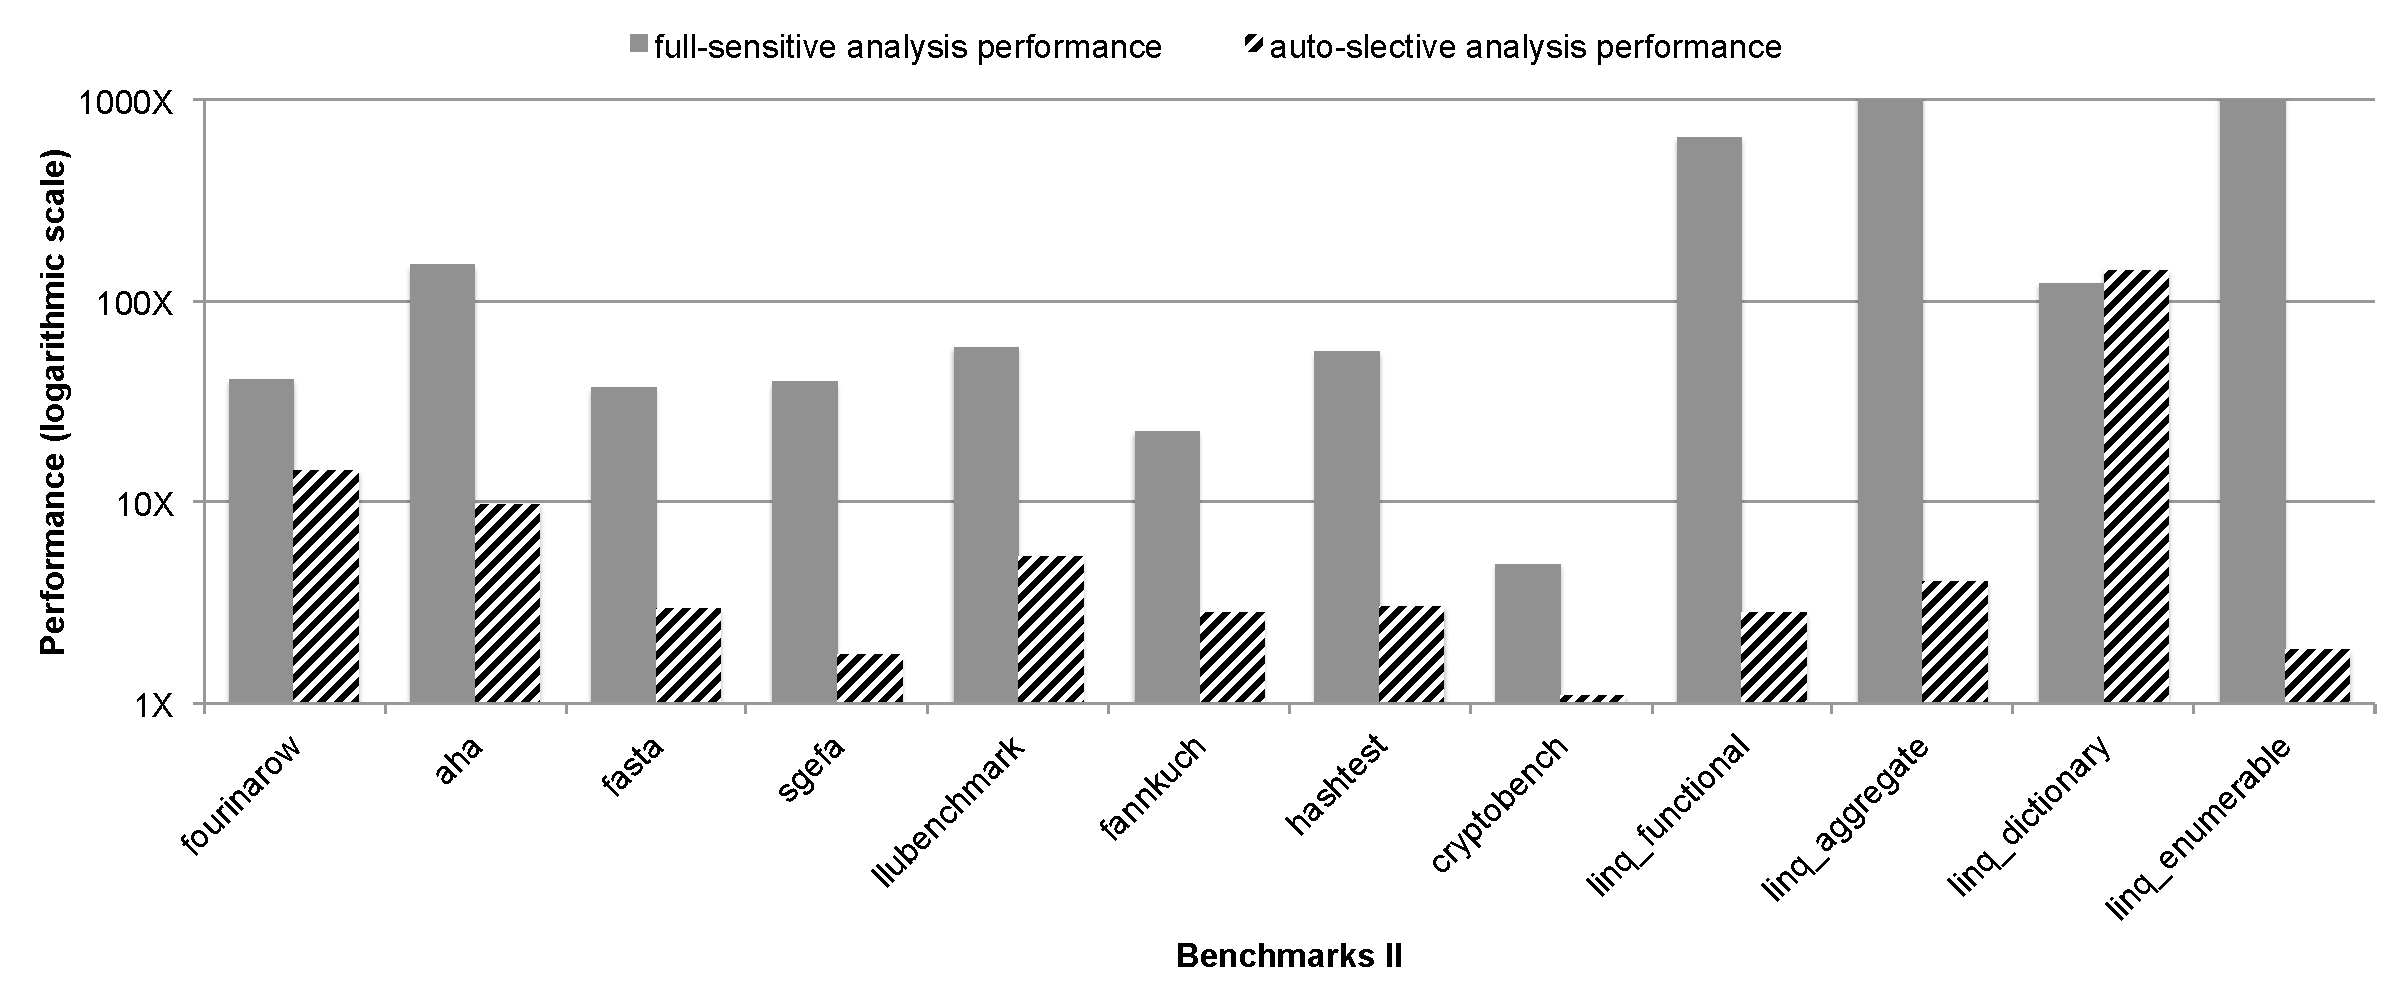
\includegraphics[width=2\columnwidth]{b2-performance}
\caption{\textmd{Benchmarks II performance results.}}
\vspace{-6pt}
\label{fig:b2-performance}
%\vspace{-6pt}
\end{figure*}

In Figure \ref{fig:b2-performance}, the {\it full-sensitive} analysis performs significantly worse than the 0-1-CFA analysis for all the benchmark programs. It could not finish analyzing {\it linq\_aggregate} and {\it linq\_enumerable} under the time budget of 10 minutes; therefore, the incomplete points-to results of these two programs were obtained after the timeout for comparison. The {\it full-sensitive} analysis is at least two orders of magnitude slower for another three program (i.e.,  {\it linq\_functional}, {\it aha}, and {\it linq\_dictionary}) and is between 23 (for {\it fannkuch}) and 60 (for {\it llubenchmark}) times slower for six programs than the 0-1-CFA analysis. For example, it takes less than one second for the 0-1-CFA analysis to finish analyzing {\it linq\_functional}, while the {\it full-sensitive} analysis needs almost 7 minutes to complete analyzing the same program. Despite of the fact that the {\it full-sensitive} analysis often results in relatively significant precision improvement (e.g., 28\% for {\it linq\_functional}), the performance issues outweigh the benefits of this whole-program combined context-sensitive analysis in many cases.

%, for 4 programs (i.e., {\it fourinarow}, {\it aha}, {\it sgefa} and {\it llubenchmark}) about 100 times slower and another 5 programs ({\it frannkuch}, {\it hashtest}, {\it linq\_aggregate}, {\it linq\_dictionary} and {\it linq\_enumerable}) about an order of magnitude slower. For example, it takes less than one second for the 0-1-CFA analysis to finish analyzing {\it fourinarow}, while the {\it whole-combined} analysis needs about 2 minutes to complete analyzing the same program. Despite of the fact that the {\it whole-combined} analysis often results in relatively significant precision improvement (e.g., 19.6\% for {\it fourinarow}), the performance issues outweigh the benefits of this whole-program combined context-sensitive analysis in many cases.

On the other hand, the {\it auto-selective} analysis is capable of analyzing the benchmarks under the same order of magnitude as the 0-1-CFA analysis for all but three programs (i.e., {\it fourinarow}, {\it aha} and {\it linq\_dictionary}). For example, the {\it auto-selective} analysis improves the precision over the 0-1-CFA analysis by 59\% for {\it cryptobench} and it also finishes analyzing this program almost as fast as the 0-1-CFA analysis. In most cases, the {\it auto-selective} analysis results in a much better balance between performance and precision than the {\it full-sensitive} analysis (e.g., the {\it full-sensitive} analysis is 65\% more precise but performs 5 times slower than the 0-1-CFA analysis for {\it cryptobench}). For three programs the {\it auto-selective} analysis performs more than 10 times slower than the 0-1-CFA analysis (i.e., 10, 15 and 143 times slower for {\it aha}, {\it fourinarow} and {\it linq\_dictionary}, respectively), the {\it auto-selective} analysis is still an order of magnitude faster than the {\it full-sensitive} analysis for {\it aha} and about 3 times faster than the {\it full-sensitive} analysis for {\it fourinarow}. An outlier is the performance of the {\it auto-selective} analysis for {\it linq\_dictionary}, which is similar to the {\it full-sensitive} analysis in performance for {\it linq\_dictionary}, indicating the {\it auto-selective} analysis may have applied expensive context sensitivity on a set of functions that result in performance overhead. Nevertheless, the {\it auto-selective} analysis has achieved significantly better performance than the {\it full-sensitive} analysis for most of the programs in Benchmarks II.

Our localization algorithm identifies between 6\% (for {\it fourinarow}) to 27\% (for {\it linq\_aggregate}) of the functions as the sources of precision loss, with an average of 13\% of the functions over all the programs in Benchmarks II, a relatively small fraction. Our improvement suggestion algorithm recommends 72\%, 25\%, and 3\% of all the root cause functions in Benchmarks II to apply a combined context-sensitive analysis, a single context-sensitive analysis and a context-insensitive analysis, respectively.

In summary, the {\it auto-selective} analysis obtains similar precision results to the {\it full-sensitive} analysis that improves the precision of the 0-1-CFA analysis; moreover, the {\it auto-selective} analysis' performance is significantly better than the whole-program combined fully context-sensitive analysis. This result suggests that our localization algorithm can accurately identify the small fraction of functions as root causes and our improvement suggestion algorithm can suggest the appropriate context sensitivity that benefit the results both in performance and precision for Benchmarks II.

%\subsection{Case Study}
%\label{case-study}

%\subsection{Discussion}